\documentclass[../../../../../../../dd.tex]{subfiles}

\begin{document}

	\subsubsection{Requests and Reservations Manager}
		This component contains all the classes that are in charge to add/remove ride requests and ride reservations. In this component are also contained classes that check the database to find not handled requests or reservations that have to be handled.
		\\
		Here are contained these main classes:
		\\
		\begin{itemize}
			\item \textbf{Taxi Request Adder:} This sub-component is in charge to create the data for a new request entry in the database and send them to the Data Tier calling the Database Manager function that add a new Ride in the Database.
			These data are Customer ID, Customer Position, Customer Zone, Request Time and Date.

			\item \textbf{Taxi Reservation Manager:} This sub-component is in charge to create the data for a new taxi reservation entry in the database and send them to the Data Tier calling the Database Manager function, that add a new Reservation in the Database.
			These data are Customer ID, starting position, ending position, request time and date.
			\\This sub-component is also in charge to send data about the Reservations to the Customers and to delete one Reservation if it can be done.

			\item \textbf{Taxi Allocator:} This sub-component is in charge to check if there are reservations or ride requests that are not been handled yet and handle them.
			This means that Taxi Allocator has to communicate with Zones Manager (to get the first available Taxi Driver), with the IO Manager (to notify Customers and Taxi Drivers) and with the Database Manager (to get reservations and requests to allocate).

		\end{itemize}

		\begin{figure}[H]
				\centering
				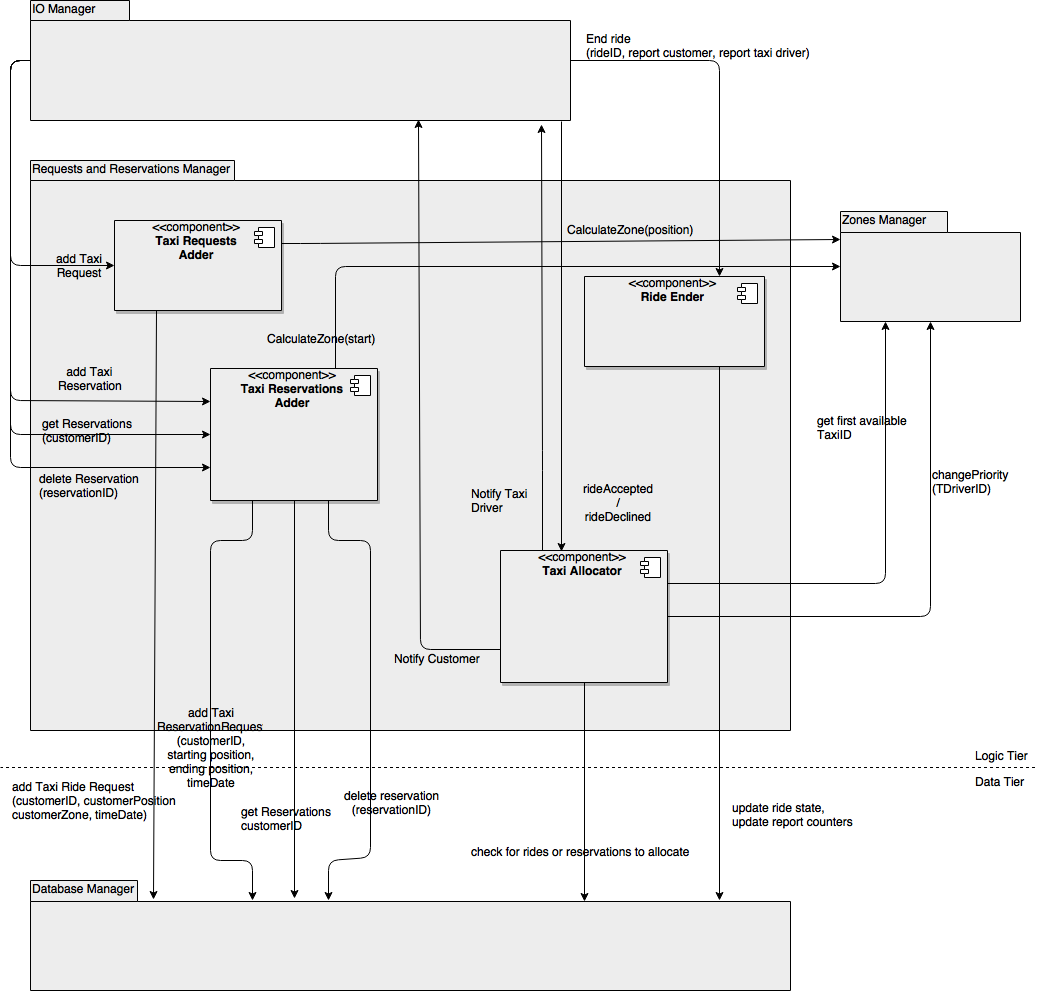
\includegraphics[width=\textwidth, scale=0.5]{../images/RequestsAndReservationsManager.png}
			\caption{Requests And Reservations Manager Structure}\label{fig:RequestsAndReservationsManager}
		\end{figure}
	
\end{document}